\chapter{Crittografia Simmetrica}

\begin{figure}[h]
    \centering
    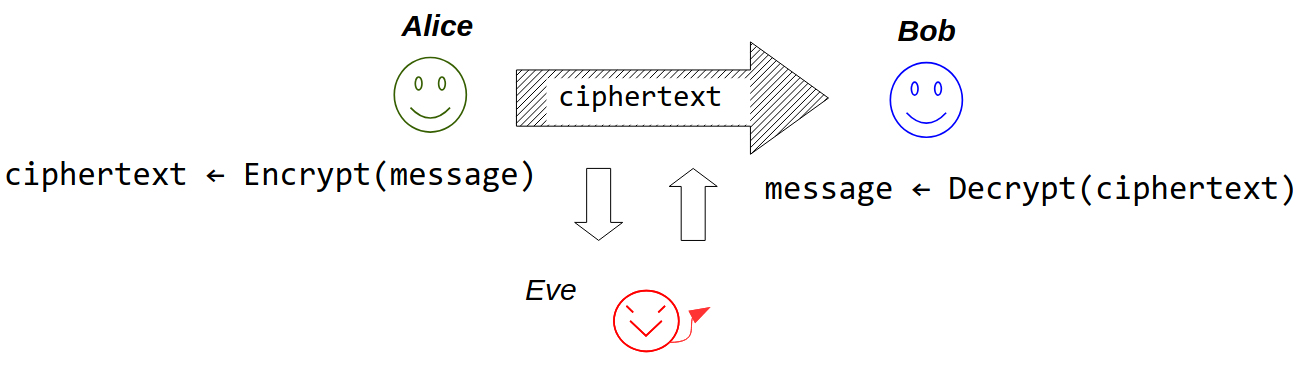
\includegraphics[width=\textwidth]{img/crypto_symm_1.png}
\end{figure}

Le garanzie di sicurezze che si cercano di mantenere sono:
\begin{itemize}[nosep]
    \item \textbf{confidenzialità}: Eve non può accedere a nessuna della informazioni sul messaggio.
    \item \textbf{autenticazione}: Bob può verificare se il messaggio non è stato inviato da Alice, viene anche chiamata \textbf{\textit{data orgin authenticity}} nel contesto della comunicazioni e implica anche la protezione contro modifiche illegittime (\textbf{integrità}).
\end{itemize}